\documentclass{article}
\usepackage{iclr2027_conference,times}

\usepackage{amsmath,amssymb,amsthm}
\usepackage{booktabs}
\usepackage{multirow}
\usepackage{graphicx}
\usepackage{capt-of} % side captions via \captionof
\usepackage{microtype}
\usepackage{xcolor}
\usepackage{tikz}
\usetikzlibrary{arrows.meta,positioning,decorations.pathmorphing}
\usepackage[colorlinks=true,linkcolor=blue,citecolor=blue]{hyperref}
\usepackage{url}

\usepackage{algorithm}
\usepackage{algpseudocode}
\usepackage{paralist}

% -------------------------------- macros --
\newcommand{\E}{\mathbb{E}}
\newcommand{\ind}[1]{\mathbf{1}\!\left[#1\right]}
\newcommand{\sg}{\mathrm{sg}}
\newcommand{\cube}{c}
\newcommand{\Reach}{\mathrm{reach}}
\newcommand{\Visit}{\mathrm{visit}}
\newcommand{\Nhat}{\hat N}

\newtheorem{proposition}{Proposition}


\title{Region-Based Successor Measures for Offline Robot Manipulation}
\author{Anonymous}

% Uncomment for the camera-ready version.
% \iclrfinalcopy

\begin{document}
\maketitle

% ============================================================================
\section{Preliminaries}
\label{sec:prelim}

\paragraph{Successor measures.}
We consider a Markov decision process with state space $\mathcal{S}$, action space $\mathcal{A}$, transition kernel $P$, and discount factor $\gamma\in(0,1)$.
The successor measure of a policy $\pi$ is its discounted future state occupancy, viewed as a measure over measurable sets $X\subseteq\mathcal{S}$:
\begin{equation}
\label{eq:sm}
M^{\pi}(s,a,X)
=
\E_{\pi}\!\left[
\sum_{t\ge0}\gamma^{t}\ind{s_{t+1}\in X}
\,\middle|\,
s_{0}=s,a_{0}=a
\right].
\end{equation}
For any reward function $r$, the corresponding action value is obtained by integrating the reward against this measure:
\begin{equation}
Q_r^{\pi}(s,a)=\int r(x)\,dM^{\pi}(s,a,x).
\end{equation}
Successor measures therefore separate learning the environment dynamics from specifying the downstream reward \citep{dayan1993improving,blier2021learning}.
Their Bellman equation, written over sets, is
\begin{equation}
\label{eq:density-bellman}
M^{\pi_z}(s,a,X)
=
P(s'\in X\mid s,a)
+
\gamma\,\E_{s',a'\sim\pi_z}\!\left[M^{\pi_z}(s',a',X)\right].
\end{equation}

\paragraph{Forward-backward representations.}
Forward-backward representations \citep{touati2021learning,touati2023does} factorize the successor measure's density with respect to a reference distribution $\rho$, which is typically the dataset marginal:
\begin{equation}
\label{eq:fb}
M^{\pi_z}(s,a,X)
\approx
\int_X F(s,a,z)^{\top}\psi(x)\,d\rho(x).
\end{equation}
Here $z$ is a task vector indexing a family of policies $\pi_z$, while $x$ is an independently queried future state.
The forward representation $F(s,a,z)$ describes the future occupancy induced by $\pi_z$, and the backward representation $\psi(x)$ embeds the queried state.

At test time, a reward observed on dataset states is converted to a task vector by reward inference, and the agent acts greedily on the resulting value estimate without further training.
In its basic form,
\begin{equation}
\label{eq:fb-reward-inference}
z_r\propto\E_{x\sim\rho}[r(x)\psi(x)],
\end{equation}
\begin{equation}
Q_r(s,a)\approx F(s,a,z_r)^{\top}z_r.
\end{equation}
This independent query is what allows one learned model to support rewards that are not expressible as a single goal.

\paragraph{FB training objective.}
Let
\begin{equation}
m_z(s,a,x)=F(s,a,z)^{\top}\psi(x)
\end{equation}
denote the learned successor density.
Standard FB uses the surrogate loss \citep{touati2021learning}
\begin{equation}
\label{eq:fb-loss}
\mathcal{L}_{\mathrm{FB}}
=
\tfrac{1}{2}\E_{x\sim\rho}\big[(m_z-\gamma\bar m_z)^2\big]
-
\E\big[m_z(s,a,s')-\gamma\bar m_z(s,a,s')\big]
+
\lambda_{\mathrm{ortho}}\mathcal{L}_{\mathrm{ortho}}.
\end{equation}
Random query states receive a squared residual, while the observed successor receives a linear positive term.
The orthonormality regularizer constrains the geometry and scale of the backward representation.

\section{Why manipulation play is different}
\label{sec:play-structure}

\subsection{Manipulation play concentrates occupancy at resting configurations}
\label{sec:playdata}

Successor measures count discounted future visits.
Whether these visits provide a useful control signal depends on which part of the state defines the task.

In locomotion and maze navigation, the goal-relevant variable is usually the agent's own position or configuration.
As the agent moves through the environment, it also moves through the goal space.
A trajectory may revisit a location, but it usually occupies each location only briefly while traversing a path.

Manipulation play has a different structure.
The goal-relevant variable is an object's configuration, while most of the state describes the robot and the surrounding scene.
The robot can approach an object, pause, release it, or prepare another grasp without changing the object's position.
Consequently, the full state can continue changing while the goal-relevant outcome remains fixed, and trajectories spend long contiguous periods at a small number of resting object configurations.

This persistence is substantial in \texttt{cube-single-play-v0}.
The cube position is unchanged on $48\%$ of transitions, and stationary runs have a median length of $44$ steps.
A $4$\,cm region around a random dataset state contains only $1.3\%$ of the dataset, yet a trajectory accumulates approximately $25$--$31$ discounted visits in that region after first entering it, out of a maximum of
\begin{equation}
1/(1-\gamma)=100
\end{equation}
for
\begin{equation}
\gamma=0.99.
\end{equation}
Thus, most of the successor measure's magnitude is accumulated after the object has already reached a configuration.

\begin{figure}[t]
\centering
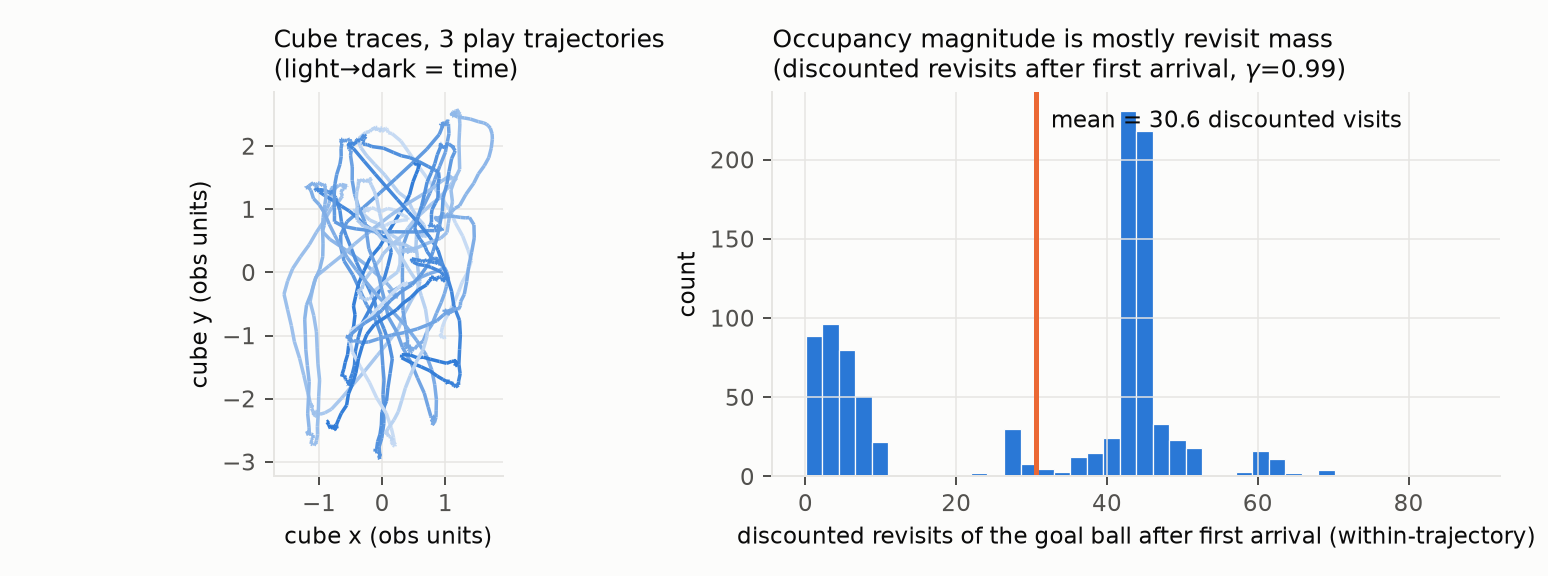
\includegraphics[width=0.95\textwidth]{figures/playdata.png}
\caption{Manipulation play concentrates occupancy where the object rests.
\emph{Left:} cube traces of three play trajectories alternate between transport and long stationary periods.
\emph{Right:} discounted occupancy of a $4$\,cm goal region accumulated after its first arrival (within-trajectory Monte Carlo, $\gamma=0.99$).
The mean is $30.6$ discounted visits out of a maximum of $100$, so most of the successor measure's magnitude comes from post-arrival occupancy rather than reaching.}
\label{fig:playdata}
\end{figure}

The same structure strengthens with additional objects because play generally manipulates one object while the others remain fixed.
On \texttt{cube-double-play-v0}, each cube is stationary on $72\%$ of transitions and post-arrival occupancy of the conjunctive goal region averages $32$ discounted visits.
On \texttt{scene-play-v0}, the drawer and window are stationary on $91\%$ of transitions, the buttons on $99.6\%$, and post-arrival occupancy averages $37$ visits.
Manipulation play therefore induces concentrated occupancy in the variables used to specify downstream tasks.

\subsection{Reaching a region and occupying it are different signals}
\label{sec:reach-vs-visit}

Let
\begin{equation}
\cube(s)
\end{equation}
denote the object configuration used to define goals, and let
\begin{equation}
B_\epsilon(g)=\{s:\|\cube(s)-\cube(g)\|\le\epsilon\}
\label{eq:goal-region}
\end{equation}
be the region associated with goal $g$.
Define the region indicator
\begin{equation}
h(s',g)=\ind{s'\in B_\epsilon(g)}=\ind{\|\cube(s')-\cube(g)\|\le\epsilon}.
\label{eq:hit}
\end{equation}

The discounted occupancy of this region under a policy $\pi$ is
\begin{equation}
M^{\Visit}(s,a,g)
=
\E_\pi\!\left[
\sum_{t\ge0}\gamma^t h(s_{t+1},g)
\,\middle|\,
s_0=s,a_0=a
\right].
\label{eq:region-occupancy}
\end{equation}
Let
\begin{equation}
T_g=\min\{t\ge0:s_{t+1}\in B_\epsilon(g)\}
\end{equation}
denote the first hitting time.
The region occupancy separates into first arrival and occupancy after arrival:
\begin{align}
M^{\Visit}(s,a,g)
&=
\underbrace{
\E_\pi\!\left[\gamma^{T_g}\ind{T_g<\infty}\right]
}_{Q^{\Reach}(s,a,g)}
\nonumber\\
&\quad+
\underbrace{
\E_\pi\!\left[
\ind{T_g<\infty}
\sum_{t>T_g}\gamma^t h(s_{t+1},g)
\right]
}_{\text{post-arrival occupancy}}.
\label{eq:occupancy-decomposition}
\end{align}

The first term asks whether the policy reaches the region and how quickly it does so.
It is the standard goal-conditioned value under the absorbing convention \citep{kaelbling1993learning,andrychowicz2017hindsight}.
The second term asks how long the policy remains in, or returns to, the region after first arrival.

These quantities serve different downstream objectives.
Goal-conditioned manipulation benchmarks evaluate whether an object reaches a target region, so visits after the first hit provide no additional success.
General reward transfer requires the complete discounted occupancy because a reward may be collected repeatedly.
A successor measure is therefore the correct object for reward integration, but it contains more than the first-arrival signal needed for goal-reaching control.

On manipulation play, the post-arrival component dominates numerically.
A regressor given only the goal predicts post-arrival occupancy with rank correlation $0.60$--$0.63$, whereas the reachability value predicts it at only $0.06$.
This suggests that much of the successor measure's magnitude is determined by where objects tend to rest, while more of the action-selection information for first-arrival control lies in the smaller reachability component.
The central problem is therefore that manipulation play data makes its largest component weakly aligned with reaching and highly concentrated around resting configurations.

\subsection{Why pointwise density estimation is problematic}
\label{sec:failure}

The preceding issue concerns what dominates the successor measure.
A second issue concerns how FB represents that measure.
FB models occupancy as a pointwise density with respect to the dataset distribution.
Under deterministic continuous dynamics, however, the one-step transition is a point mass and has no finite density with respect to a distribution that assigns zero probability to individual states.

\begin{proposition}[Point densities are singular; region targets are bounded]
\label{prop:fixed-points}
Suppose the dynamics are deterministic,
\begin{equation}
s'=f(s,a),
\end{equation}
and the reference distribution $\rho$ is non-atomic.
Then the one-step transition measure $\delta_{f(s,a)}$ has no density with respect to $\rho$.
For any measurable region $G$, however,
\begin{equation}
P(G\mid s,a)=\ind{f(s,a)\in G}\in\{0,1\},
\end{equation}
and the absorbing and non-absorbing region Bellman operators obtained from Equation~\ref{eq:density-bellman} are $\gamma$-contractions on bounded functions.
(Proof in Appendix~\ref{app:derivations}.)
\end{proposition}

The singularity follows from deterministic continuous dynamics and is not unique to manipulation.
A deterministic transition places unit mass at one state, while a non-atomic reference distribution assigns zero mass to every individual state, so no finite density with respect to $\rho$ represents the one-step target.
Manipulation play amplifies the practical problem because its successor measure concentrates around persistent object configurations.
Long resting segments repeatedly supply positive examples from this narrow part of the goal space while the target remains singular.

Equation~\ref{eq:fb-loss} makes the resulting effect on optimization explicit.
Random query states receive a squared residual, while the observed successor receives a term that rewards increasing its score \citep{eysenbach2022contrastive}.
The positive term is linear, so increasing the matched score always reduces the loss, at any scale.
On manipulation play, long resting segments repeatedly reinforce successors with the same or nearby object configurations.
The orthonormality penalty on $\psi$ is then the only part of the objective that indirectly constrains scale.

\section{Region-based successor learning}
\label{sec:bounded}

Our method follows a simple progression.
We first learn which actions reach a goal region, then continue training the same model to predict where the resulting policy spends time.
This requires two changes to standard FB: replacing pointwise density queries with finite-region events, and separating reachability from occupancy through two training phases.

\begin{figure}[htb]
\centering
\begin{minipage}[c]{0.60\textwidth}
\centering
\includegraphics[width=\textwidth]{\detokenize{figures/Factored-FB (1).png}}
\end{minipage}\hfill
\begin{minipage}[c]{0.36\textwidth}
\raggedright
\captionof{figure}{Forward-backward (FB) representations factorize the successor measure into a forward embedding $F(s,a,z)$ and a backward state embedding $\psi(x)$.
The independent query $x$ allows one learned model to evaluate rewards that are not expressible as a single goal.}
\label{fig:factored-fb}
\end{minipage}
\end{figure}


\subsection{Bounded region targets}
\label{sec:regions}

Instead of predicting occupancy at an exact state $g$, we predict occupancy of a neighborhood
\begin{equation}
B_\epsilon(g)
=
\{x:\|\cube(x)-\cube(g)\|\leq\epsilon\}.
\end{equation}
For a transition \((s,a,s'),\), its immediate contribution is the bounded event
\begin{equation}
\label{eq:hit}
h(s',g)
=
\ind{s'\in B_\epsilon(g)}
\in\{0,1\}.
\end{equation}
This replaces the singular point-density target with an ordinary sparse goal-conditioned reward.

We retain the FB factorization.
A goal encoder \( \psi_\phi(g)\), forward network \(F_\theta(s,a,z)\),  and task-conditioned actor \(\pi_\omega(s,z)\) define
\begin{equation}
    \label{eq:region-factorization}
    M_\theta(s,a,z,g) = F_\theta(s,a,z)^\top\psi_\phi(g),
\end{equation}
where $z$ specifies the policy and $g$ specifies the queried region.

For a batch of transitions $\{(s_i,a_i,s'_i)\}_{i=1}^n$ and query goals $\{g_j\}_{j=1}^n,$ we train all state-goal pairs using
\begin{equation}
\label{eq:matrix-loss}
\mathcal{L}_{\mathrm{TD}} = \frac{1}{n^2} \sum_{i,j} \left( M_\theta(s_i,a_i,z_j,g_j)-y_{ij} \right)^2.
\end{equation}
The binary immediate target fixes the value scale, removing the linear positive term and orthonormality constraint used by the FB density objective.

\subsection{Two-stage training}
\label{sec:two-stage}

The two phases use the same architecture but learn different quantities.

\paragraph{Phase 1: goal-conditioned reachability.}
We tie the policy task to the queried goal, $z_j=z_{g_j},$ and use the absorbing target
\begin{equation}
\label{eq:phase1-target}
y^{\Reach}_{ij} = h_{ij} + \gamma(1-h_{ij}) \bar Q^{\Reach} \left( s'_i, \pi_{\bar\omega}(s'_i,z_{g_j}), g_j \right),
\end{equation}
where $h_{ij}=h(s'_i,g_j)$.
The factor $(1-h_{ij})$ stops the backup after the first hit.
We jointly optimize $F_\theta$, $\psi_\phi$, and $\pi_\omega$.
The fixed point is
\begin{equation}
Q^{\Reach}(s,a,g) = \E\!\left[ \gamma^{T_g}\ind{T_g<\infty} \right] \in[0,1].
\end{equation}

\paragraph{Phase 2: policy-conditioned occupancy.}
We initialize from phase 1, freeze $\psi_\phi$, and sample the policy task $z_j$ independently of the query goal $g_j$.
We then use the non-absorbing target
\begin{equation}
\label{eq:phase2-target}
y^{\Visit}_{ij} = h_{ij} + \gamma \bar M^{\Visit} \left( s'_i, \pi_{\bar\omega}(s'_i,z_j), z_j, g_j \right).
\end{equation}
We update $F_\theta$ and $\pi_\omega$ while keeping $\psi_\phi$ fixed.
The fixed point is
\begin{equation}
M^{\Visit}(s,a,z,g) = \E_{\pi_z}\!\left[ \sum_{t\geq0} \gamma^t h(s_{t+1},g) \right] \in \left[ 0,\frac{1}{1-\gamma} \right].
\end{equation}

Phase 1 learns which actions reach a region, serving as an initialization. 
Phase 2 learns which regions each task-conditioned policy occupies by directly optimizing the occupancy Bellman equation rather than factorizing occupancy into reachability and recurrence
(Appendix~\ref{app:twostage}).
Freezing $\psi_\phi$ preserves the goal representation learned in phase 1; Section~\ref{sec:frozenrep} evaluates this choice.

\begin{algorithm}[t]
\caption{Region-based successor learning}
\label{alg:region-successor}
\small
\begin{algorithmic}[1]
\Require Offline dataset $\mathcal{D}$; networks $F_\theta$, $\psi_\phi$, $\pi_\omega$
\State Initialize networks and target networks
\For{phase-1 gradient steps}
    \State Sample transitions $\{(s_i,a_i,s'_i)\}$ and goals $\{g_j\}$
    \State Set each policy task to its query goal: $z_j\gets z_{g_j}$
    \State Compute $h_{ij}=\ind{s'_i\in B_\epsilon(g_j)}$
    \State Form reachability targets using Equation~\ref{eq:phase1-target}
    \State Update $\theta$, $\phi$, and $\omega$ using Equation~\ref{eq:matrix-loss}
\EndFor
\State Freeze the goal encoder $\psi_\phi$
\For{phase-2 gradient steps}
    \State Sample transitions, policy tasks $\{z_j\}$, and independent goals $\{g_j\}$
    \State Compute $h_{ij}=\ind{s'_i\in B_\epsilon(g_j)}$
    \State Form occupancy targets using Equation~\ref{eq:phase2-target}
    \State Update $\theta$ and $\omega$ using Equation~\ref{eq:matrix-loss}
\EndFor
\State \Return $F_\theta$, $\psi_\phi$, and $\pi_\omega$
\end{algorithmic}
\end{algorithm}

\subsection{Test-time reward inference}
\label{sec:readout}

The model predicts region mass rather than pointwise density.
Let
\begin{equation}
N_\epsilon(g) = \rho(B_\epsilon(g))
\end{equation}
denote the probability mass of the region under the dataset distribution.
When the successor density is approximately constant inside the region,
\begin{equation}
M^\pi(s,a,B_\epsilon(g)) \approx m^\pi(s,a,g)N_\epsilon(g).
\end{equation}
Reward values and task embeddings are therefore recovered as
\begin{equation}
\label{eq:readout}
Q_r^\pi(s,a) \approx \E_{g\sim\rho} \left[ \frac{r(g)}{N_\epsilon(g)} M^\pi(s,a,B_\epsilon(g)) \right],
\end{equation}
\begin{equation}
z_r = \E_{g\sim\rho} \left[ \frac{r(g)}{N_\epsilon(g)} \psi_\phi(g) \right].
\end{equation}
We estimate $N_\epsilon(g)$ using a learned head $\Nhat$.
Because $z_r$ averages multiple goal embeddings, phase-2 task sampling also includes reward-induced embeddings; Section~\ref{sec:rq2} evaluates this addition.



\section{Experiments}
\label{sec:experiments}

We first isolate whether the observed failure arises from the representation or from the point-density objective itself (Section~\ref{sec:frozenrep}).
We then ask four questions: 
\begin{inparaenum}
    \item does region-based TD restore goal-conditioned control (Section~\ref{sec:rq1});
    \item does occupancy fine-tuning improve held-out reward transfer (Section~\ref{sec:rq2});
    \item does the learned function satisfy measure properties (Section~\ref{sec:rq3}); and
    \item  does the approach extend to multi-object manipulation (Section~\ref{sec:rq4})?
\end{inparaenum}

\paragraph{Setting.}
We use OGBench state-based manipulation \citep{park2024ogbench}, primarily \texttt{cube-single-play-v0}: a $6$-DoF arm, one cube, $28$-dimensional states, and $10^6$ offline transitions of scripted play that repeatedly picks the cube up, carries it, and sets it down.
No benchmark reward labels are used to fit any of our objectives.
The method is given a state abstraction $\cube(x)\in\mathbb{R}^3$ (cube position) and a radius $\epsilon=4\,\text{cm},$ which define goal regions
\begin{equation}
    B_\epsilon(g)=\{x:\|\cube(x)-\cube(g)\|\le\epsilon\}.
\end{equation}
This is a substantive assumption, three of twenty-eight state dimensions, at the benchmark's own tolerance, and we quantify what it contributes in \S\ref{sec:results}.

\paragraph{Protocol.}
Unless stated otherwise: rank-$50$ bilinear critic $F^\top\psi,$, twin heads with a minimum target, $\gamma=0.99,$ hindsight-relabeled batch goals (a batch of $n$ transitions yields an $n\times n$ matrix of state-goal pairs), a flow-matching behavior-cloning actor with one-step distillation, $500$k gradient steps, $3$ seeds per cell.
\emph{Task success} means the benchmark's goal-conditioned evaluation, averaged over its five tasks with $50$ episodes each.
Measure-side evaluations (Monte-Carlo occupancy comparisons, reward-transfer protocols) are defined where they are used.

\subsection{Does the density objective fail on a fixed representation?}
\label{sec:frozenrep}

We first rule out representation quality as the explanation for FB's failure.
We freeze $\psi$ at a checkpoint that already supports $0.97$ task success and train only the density estimator on top of it.
Without the orthonormality term, the critic's scale grows from $154$ to $5.4\times10^4$ within $65$k steps and mean success decreases monotonically from $0.98$ to $0.42$ by $100$k steps, averaged over three seeds (Figure~\ref{fig:diverge}).
Allowing $\psi$ to train accelerates the collapse, from $0.97$ to $0.07$ by $50$k steps.
With the orthonormality term, the scale remains bounded but success reaches only $0.225$; 
a fully tuned FB implementation reaches approximately $0.42$, compared with $0.928$ for the architecture-matched GCIQL baseline.
Therefore, the estimator, is the bottleneck.

\begin{figure}[t]
\centering
\begin{minipage}[t]{0.48\textwidth}
\centering
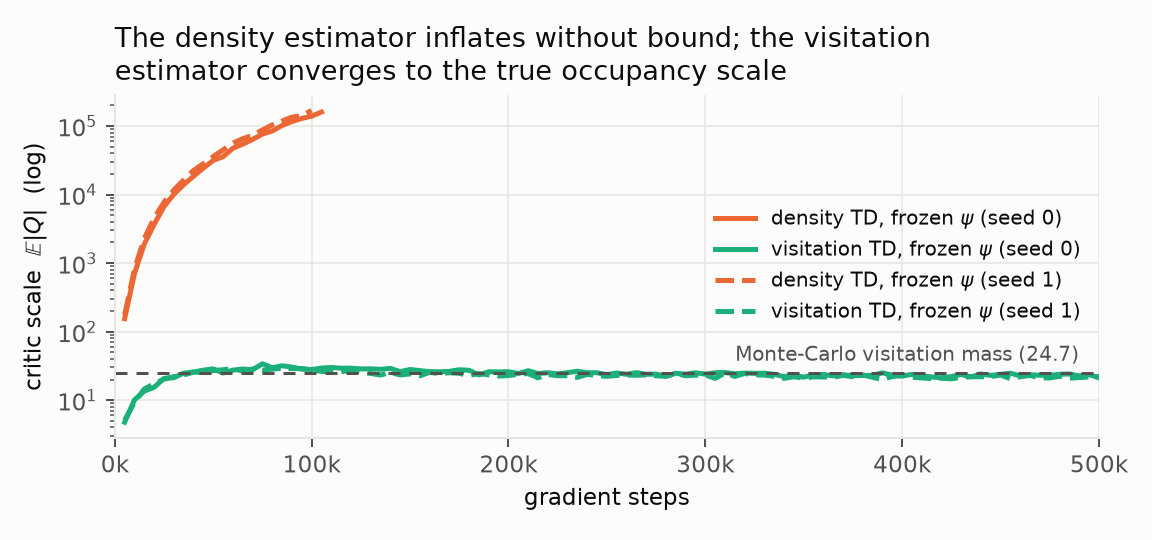
\includegraphics[width=\textwidth]{figures/scale_divergence.png}
\end{minipage}\hfill
\begin{minipage}[t]{0.48\textwidth}
\centering
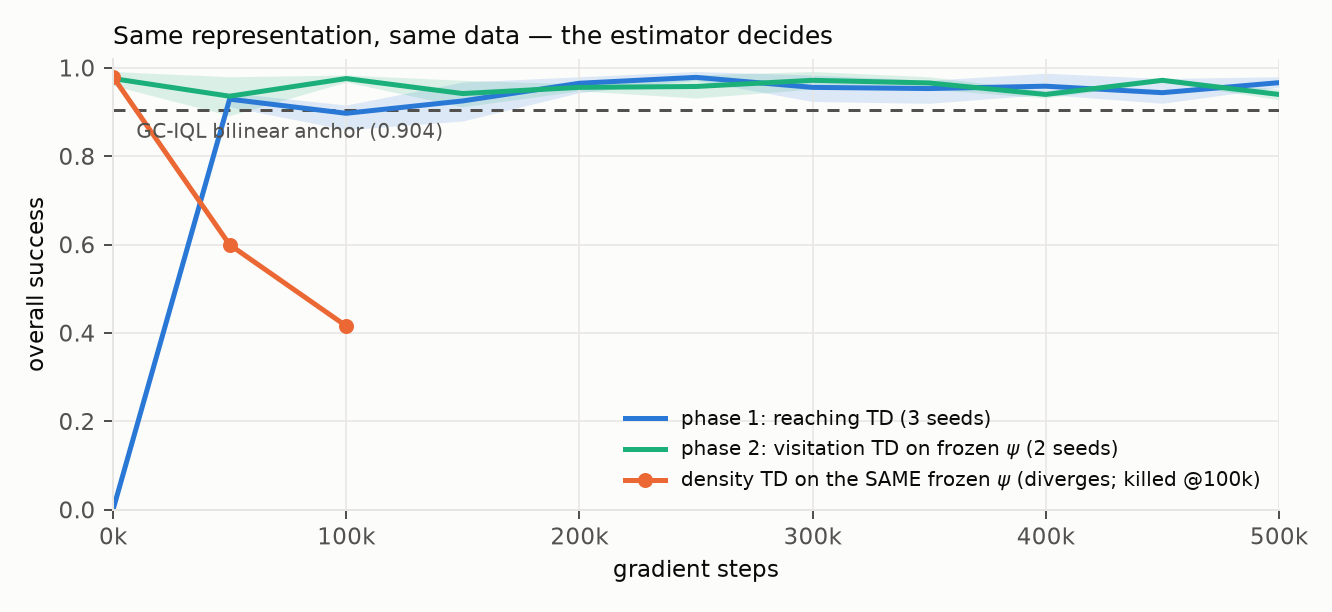
\includegraphics[width=\textwidth]{figures/2_curves.png}
\end{minipage}
\caption{One frozen representation, three objectives.
\emph{Left:} critic scale $\E|Q|$ on a frozen goal embedding $\psi$.
Without the orthonormality term, the density objective grows without bound because its linear positive term always rewards a larger matched score.
The region-indicator objective converges to the Monte-Carlo estimate of the true discounted occupancy because every TD target is finite.
\emph{Right:} task success under the same frozen embedding.
The reachability and region-occupancy objectives remain stable, while the density objective degrades immediately.}
\label{fig:diverge}
\end{figure}

\subsection{Does region-based TD restore goal-conditioned control?}
\label{sec:rq1}\label{sec:results}

Table~\ref{tab:main} compares goal-reaching success on the three environments, against the OGBench reference implementations and against baselines re-implemented in the matched architecture.

\begin{table}[t]
\centering\small
\begin{tabular}{l ccc}
\toprule
Method & \texttt{cube-s} & \texttt{cube-d} & \texttt{scene} \\
\midrule
\multicolumn{4}{l}{\emph{reported by OGBench \citep{park2024ogbench}, reference implementations, $8$ seeds}} \\
GCBC   & $0.06$ & $0.01$ & $0.05$ \\
GCIVL  & $0.53$ & $0.36$ & $0.42$ \\
GCIQL  & $0.68$ & $0.40$ & $0.51$ \\
CRL    & $0.19$ & $0.10$ & $0.19$ \\
HIQL   & $0.15$ & $0.06$ & $0.38$ \\
\midrule
\multicolumn{4}{l}{\emph{architecture-matched comparison, same data, flow-BC actor, bilinear rank-$50$ critic, $2$-$10$ seeds}} \\
GCIQL baseline           & $0.928$ & $0.265$ & $0.281$ \\
CRL                      & $0.311$ & ,     & ,     \\
Tuned FB                 & $0.42$  & ,     & $0.047$ \\
FB (reference reimpl.)   & $0.532$ & ,     & ,     \\
FB loss on regions       & $0.284$ & ,     & ,     \\
\midrule
Reachability value (phase 1) & $\mathbf{0.967}$ & $\mathbf{0.549}$ & $\mathbf{0.484}$ \\
Region occupancy (phase 2)   & $0.940$ & $0.358$ & $0.342$ \\
\bottomrule
\end{tabular}
\caption{Goal-reaching success ($500$k steps; five tasks, $50$ episodes each).
The degenerate \texttt{puzzle-3x3}, where the matched implementation solves only task 1, is omitted.
The top block quotes the OGBench paper's reference implementations (their architectures and tuning); the middle block re-implements baselines in the matched architecture. Dashes: not run.}
\label{tab:main}
\end{table}

\paragraph{Region-based TD restores goal-conditioned control.}
The reachability value outperforms the architecture-matched GCIQL baseline on all three environments, with the largest improvements on \texttt{cube-double} and \texttt{scene} (Table~\ref{tab:main}).
Against OGBench's reference implementations it is the strongest evaluated method on \texttt{cube-single} and \texttt{cube-double} and comparable to reference GCIQL on \texttt{scene}.
With a bounded target, the same representation class that FB uses is competitive with the strongest evaluated baselines.

\paragraph{Successor-style baselines degrade where occupancy concentrates.}
CRL, the contrastive counterpart, scores $0.10$-$0.31$ across implementations, and FB drops to $0.047$ on \texttt{scene}, the environment where the object-at-rest concentration is strongest (\S\ref{sec:playdata}).
This pattern is consistent with the proposed mechanism, although it does not isolate it.

\paragraph{Which change is responsible?}
A $2\times2$ ablation crosses the loss form (FB's surrogate vs.\ indicator-TD) with the query support (point vs.\ region).
FB's own loss on regions reaches $0.284$ (Table~\ref{tab:main}, ``FB loss on regions''); indicator-TD with the region collapsed back to a point ($h=I$ on the batch) reaches $0.108$; the combination reaches $0.922$ (replicated in a second implementation).
Neither change suffices alone.
The region also need not be the evaluation variable: the same ball built on the \emph{end-effector} position, correlated with, but distinct from, the evaluated cube, reaches $0.823$.
The region variable therefore need not exactly match the evaluation variable, although this ablation does not establish that the choice of variable is unimportant in general.

\subsection{Does occupancy fine-tuning improve held-out reward transfer?}
\label{sec:rq2}\label{sec:reward-transfer}

Fine-tuning nearly doubles compositional-reward return, and with the two corrections below the final model reaches $1.9\times$ the mean return of the reimplemented FB baseline (Table~\ref{tab:transfer}).

\begin{table}[t]
\centering\small
\begin{tabular}{l cccc}
\toprule
Method & concentrated & broad & compositional & mean \\
\midrule
FB (reference reimpl.)  & $8.4$ & $35.4$ & $6.9$ & $17.2$ \\
FB loss on regions      & $6.4$ & $27.2$ & $5.0$ & $13.1$ \\
\midrule
Reachability value (phase 1) & $12.1$ & $27.8$ & $8.5$  & $16.8$ \\
$+$ occupancy (phase 2)      & $16.3$ & $28.5$ & $15.8$ & $20.3$ \\
$+$ reward-embedding coverage & $20.2$ & $31.5$ & $23.0$ & $24.5$ \\
$+$ measure regularizers & $\mathbf{26.1}$ & $\mathbf{41.6}$ & $\mathbf{33.0}$ & $\mathbf{32.4}$ \\
\bottomrule
\end{tabular}
\caption{Held-out reward return on \texttt{cube-single}: $48$ rewards over the cube abstraction, absolute discounted return (rewards in $[0,1]$, returns in $[0,86.6]$, behavior-policy baseline $8.1$; family means of two seeds, FB single-seed).
Concentrated $=$ balls at radii $0.4/0.8$ and Gaussians at bandwidth $0.4$; broad $=$ ball $1.6$ and Gaussian $0.8$; compositional $=$ two disjoint zones.
Rows below the rule are cumulative; goal-reaching success is unchanged by the two corrections ($0.940\to0.947$-$0.950$).}
\label{tab:transfer}
\end{table}

The rewards are functions of the supplied cube abstraction, all with values in $[0,1]$: indicator balls at radii $0.4/0.8/1.6$ (the training kernel is $0.4$), Gaussians at bandwidths $0.4/0.8$, and a two-zone reward (two disjoint balls more than $1.6$ apart, not expressible as any single goal); eight instances per family, centers drawn from dataset states.
Task vectors come from least-squares reward inference over $10^4$ relabeled dataset rows, no ridge term, no candidate search.
For per-family analysis we score control as the fraction of the gap between a random-$z$ floor and a single-goal oracle proxy; scores above $1$ mean beating that proxy, not optimality.

\paragraph{FB's return comes from broad rewards.}
FB performs best on the broad family, above our phase-1 and phase-2 models, because a $16$\,cm ball assigns reward to almost any cube displacement, and $3$-$5\times$ below the final method on the concentrated and compositional families, where the reward has structure.

\paragraph{Occupancy fine-tuning trades goal-reaching success for transfer.}
Fine-tuning reduces goal-reaching success on \texttt{cube-double} and \texttt{scene} ($-0.19$/$-0.14$; \S\ref{sec:rq4} removes this reduction) but improves reward transfer where occupancy matters: on the compositional family, which no single goal expresses, return nearly doubles.
The two corrections below raise mean return further without reducing goal-reaching success.

\paragraph{Verifying the readout weight.}
The inverse-mass weight of Equation~\ref{eq:readout} is visible in the data.
With the weight omitted, predicted returns rank well in every family (Spearman $0.62$-$0.90$) but are uniformly $0.014$-$0.030$ of the Monte-Carlo magnitude, a single family-independent scale factor.
The mean region mass, measured independently, is
\begin{equation}
\bar N=0.0137;
\end{equation}
the uncorrected predictions lie on
\begin{equation}
y=\bar N x
\end{equation}
(Appendix Figure~\ref{fig:scale}), and weighting the readout by
\begin{equation}
1/\Nhat(g)
\end{equation}
restores scale to $0.79$-$2.2$ (derivation in Appendix~\ref{app:derivations}).
The correction substantially reduces the scale error, although predictions can still differ from Monte Carlo by up to a factor of two.

\paragraph{Covering reward-induced embeddings.}
Correcting the scale does not by itself improve behavior, two-zone control \emph{falls} from $0.86$ to $0.46$ under the corrected embeddings.
This is the training-side consequence anticipated in \S\ref{sec:readout}: an inferred embedding for a broad reward is an average of many goal embeddings and lies in a part of task space that training, which samples $z$ from random directions and single-goal embeddings, never visits.
The test is to add such embeddings to training: a third task-sampling component draws a random synthetic reward and embeds it as inference would.
A \textsc{kernel} generator matches the evaluation families' functional forms; an \textsc{rff} generator shares no functional form with any evaluation family and controls for reward-family leakage (Appendix~\ref{app:rewards}).

Training on reward-induced task embeddings improves control across most reward families (Appendix Table~\ref{tab:rewardz}).
The broad indicator ball, at $0.07$ at baseline, recovers to $0.49$-$0.55$ in every arm, including \textsc{rff}, whose training rewards share no form with the evaluation family: the improvement comes from populating the averaged region of task space, not from familiarity with the test rewards.
The compositional family reaches $1.35$, exceeding the better single-zone proxy by $35\%$, which is what reward composition should produce.
Combined with the regularizers of \S\ref{sec:rq3}, the broad Gaussian improves from $0.24/0.43$ to $0.46$-$0.86$ across seeds, though it remains the least reliable family.
Task success improves alongside ($0.887\to0.950$) and calibration is intact.
Appendix Figure~\ref{fig:bandwidth} resolves the same result by the reward's spatial support.

\paragraph{What occupancy fine-tuning adds over the reachability value.}
\label{sec:cross-method}

Table~\ref{tab:transfer} answers on returns; the mechanism is visible when both policies are evaluated with the goal supplied directly: the phase-2 policy accumulates $1.13$-$2.00\times$ more reward than the phase-1 policy on identical rewards.
A reachability value is saturated once the region is entered, so its greedy policy enters and stops; a policy trained on occupancy returns to and remains in the rewarded region, exactly the post-arrival occupancy that \S\ref{sec:playdata} showed dominates this data.
The advantage disappears on the broadest rewards ($0.99$-$1.05\times$), where remaining in place earns nothing extra.
(The phase-2 checkpoint continues training from the phase-1 one, so the comparison is not iso-budget; the goal-supplied comparison is less exposed to this, but an equal-training-budget control has not been run.)

\subsection{Does the learned function satisfy measure properties?}
\label{sec:rq3}\label{sec:measure-validity}

Only partially: the estimator is coarsely calibrated but carries substantial negative mass, and removing the negative mass requires both regularizers of this section (Appendix Table~\ref{tab:measure}).
Strong task success could not have told us this: control depends mainly on the critic's action ranking at the current state.
Empirically, the goal-reaching and occupancy critics select the same greedy action on only $29.5\%/29.9\%$ of a grid of $24$ states $\times$ $150$ goals $\times$ $16$ candidate actions (chance $6.25\%$).
Task success provides evidence that the reachability critic induces an effective policy; it does not establish calibration of $M^{\Visit}$.
We therefore test the occupancy estimator directly for the properties a measure must have: calibrated set mass and non-negativity.

\subsubsection{Set-mass calibration}
\label{sec:set-calibration}

We compare predicted occupancy of random boxes against Monte-Carlo rollouts of the same policy ($32$ starts $\times$ $3$ rollouts, horizon $200$).
The learned quantity is a region mass, so converting it to a density requires dividing by the region's probability under the data distribution,
\begin{equation}
N(g)=\rho(B_\epsilon(g));
\end{equation}
a small trained head $\Nhat(g)$ estimates this factor.

At half-widths $0.8$ and $1.6$ the corrected estimate is within $10$-$23\%$ of Monte Carlo with rank correlation $0.68$-$0.85$ (Appendix Table~\ref{tab:calib}).
Two qualifications: with exact counts in the denominator, the uncorrected estimate is $1.9$-$3.2\times$ too large (the head's $+28\%$ bias partially compensates), and the smallest scale, the training kernel's own, remains $1.2$-$1.9\times$ off on every variant we trained, consistent with a resolution limit of the rank-$50$ factorization (\S\ref{sec:limitations}).

\subsubsection{Non-negativity and mass conservation}
\label{sec:nonneg}

A measure is non-negative.
The learned occupancy estimator is not: across $32$ policies and $20$k dataset goals, about half of all values are negative, the negative values carry $24$-$29\%$ of the total absolute mass at roughly a third of the positive values' magnitude, and the violation is \emph{largest} in the densest parts of goal space ($0.55$-$0.59$ of values negative in the top density quartile vs.\ $0.45$ in the bottom).
These are not boundary fluctuations; they are systematic oscillations where the regression is most constrained.
Calibration and invalidity coexist because signs cancel inside a box.

Replacing the discontinuous $0/1$ reward with a smooth kernel of matched mass changes nothing (negative fraction $0.50$-$0.52$; Appendix~\ref{app:validity}), so the violation is slack in the regression, not an artifact of the target's sharpness.

The direct correction is a one-sided penalty
\begin{equation}
\lambda\,\E[\mathrm{relu}(-M)^2].
\end{equation}
Alone, it fails, and the failure identifies the missing constraint: at $\lambda\in\{1,10\}$ the negative fraction drops to $3.1\%/0.7\%$, but total mass inflates to $2.5$-$3.6\times$ Monte Carlo.
The penalty raises negative values, and no term in the objective constrains the total.
The missing constraint is a property of the region occupancy's fixed point: because the cube is always \emph{somewhere}, averaging region mass over goals, each weighted by the inverse of its region's data probability, counts total discounted time,
\begin{equation}
\label{eq:mass-anchor}
\E_{g\sim\rho}\!\left[\frac{M(s,a,g)}{N(g)}\right]=\sum_{t\ge0}\gamma^t =\frac{1}{1-\gamma}
\end{equation}
\begin{equation}
\quad\Longrightarrow\quad \mathcal{L}_{\mathrm{mass}} = \Big((1-\gamma)\,\tfrac{1}{n}\sum\nolimits_j M_{ij}/\Nhat_j-1\Big)^{2}.
\end{equation}
The penalty holds the model to this identity (exactness conditions in Appendix~\ref{app:derivations}).
With both regularizers, sign and scale are fixed jointly (Appendix Table~\ref{tab:measure}) and task success is unchanged ($0.94$-$0.95$ vs.\ control $0.94$-$0.96$).

The measured cost: rank correlation at the middle calibration scale drops from $0.68$ to $\approx0.50$ (the coarse scale is unaffected); penalty-only runs already showed this degradation, implicating the penalty strength; a weaker penalty is under evaluation (\S\ref{sec:limitations}).

\subsection{Does the approach extend to multi-object manipulation?}
\label{sec:rq4}\label{sec:multienv-zeroshot}

Yes, with one change to how goals are sampled for the occupancy TD; the same change removes phase 2's reduction in goal-reaching success ($-0.19/-0.14$, Table~\ref{tab:main}).
On \texttt{cube-double} the trained region is a conjunction (both cubes within $\epsilon$), so a goal sampled uniformly from the dataset gives the occupancy TD a nonzero indicator at rate $0.046\%$, $28\times$ sparser than \texttt{cube-single}.
We tested the other candidate causes, kernel width, factorization rank, freezing the actor through the phase switch, and their compositions; eight pre-specified ablations, none of which improved success, and one change did: sampling the occupancy TD's goals by hindsight relabeling (future states of the same trajectory), which makes the indicator nonzero at the state-goal pairs the actor loss uses, by construction.
The cost: without an importance correction the hindsight-sampled object is no longer the successor measure with respect to the dataset distribution $\rho$ (\S\ref{sec:set-calibration}), and on \texttt{cube-single}, where dataset-sampled goals already give a nonzero indicator at $1.3\%$, the change reduces success by $0.17$-$0.24$.
It is an environment-conditional modification, not a default.

Appendix Table~\ref{tab:multienv-zeroshot} scores zero-shot control on the multi-object environments with the \texttt{cube-single} reward-transfer evaluation protocol extended to conjunctive regions (region centers drawn from visited states; the extended protocol reproduces the \texttt{cube-single} numbers of \S\ref{sec:reward-transfer} exactly).
Protocol as before: least-squares reward inference over relabeled rows, nearest-neighbor decoding of $z_r$ to a dataset goal state, the benchmark's success criteria, $25$ episodes per task at $500$k steps.

\section{Related work}
\label{sec:related}

\paragraph{Successor representations and measures.}
Successor representations predict discounted future occupancy \citep{dayan1993improving}; successor measures generalize them to continuous spaces as measures, or densities against a reference distribution \citep{blier2021learning}; FB representations factorize that density and infer tasks by least-squares reward regression \citep{touati2021learning,touati2023does}.
We keep FB's bilinear form and zero-shot protocol and change the estimand from a pointwise density, whose empirical Bellman target is a Dirac measure, to region occupancy, whose target is a sparse indicator reward, a change whose necessity is specific to data that concentrates occupancy at resting states (\S\ref{sec:playdata}).

\paragraph{Goal-conditioned RL.}
Goal-reaching values with sparse indicator rewards and hindsight relabeling are the standard objects of offline GCRL \citep{kaelbling1993learning,andrychowicz2017hindsight,kostrikov2021offline,park2023hiql}.
Contrastive RL \citep{eysenbach2022contrastive} learns classifiers of future states rather than densities, avoiding the same singular target from a different direction; our diagnosis in \S\ref{sec:playdata} makes the connection explicit, FB's surrogate is contrastive in structure but lacks the saturating positive term that keeps classification bounded.
A goal-conditioned value evaluates each goal under that goal's own policy; a successor measure retains an independent query and must support reward composition, which is why our evaluation separates reachability (task success) from the measure claim (calibration, sign, transfer).

\paragraph{Hitting values versus occupancy.}
The absorbing and non-absorbing TD targets answer different questions, whether a region is reached versus how long it is occupied.
Manipulation benchmarks score first arrival into a tolerance region, so a reachability value suffices for control; Table~\ref{tab:main} shows occupancy is nonetheless the object that improves reward transfer.

\bibliography{references}
\bibliographystyle{iclr2027_conference}

\appendix
\section{Additional experimental detail}
\label{app:detail}


\subsection{Supplementary figures and ablations}
\label{app:supplementary-figures}

\paragraph{Qualitative play trajectory.}
The generic FB factorization and the rendered play trajectory are included here for reference; the main text retains the equations and the quantitative occupancy figure.

\begin{figure}[htb]
\centering

\includegraphics[width=0.98\textwidth]{figures/0_playdata_strip.png}
\caption{One trajectory from \texttt{cube-single-play-v0}, rendered by replaying the dataset's stored simulator states.
The collector repeatedly moves the cube and leaves it at a resting configuration.
Between manipulations, the robot continues to act while the goal-relevant variable, the cube position, remains unchanged.}
\label{fig:strip}
\end{figure}


\paragraph{Reward inference and task-embedding coverage.}
The following diagnostics support the inverse-region-mass readout and the reward-induced task-embedding intervention discussed in Section~\ref{sec:rq2}.

\begin{figure}[t]
\centering
\includegraphics[width=0.46\textwidth]{figures/scale.pdf}
\caption{Predicted vs.\ Monte-Carlo return on all $48$ held-out rewards, log-log.
Uncorrected reward inference tracks $y=\bar Nx$ with $\bar N=0.0137$ the independently measured mean region mass; the $1/\Nhat$-weighted readout tracks $y=x$.}
\label{fig:scale}
\end{figure}

\begin{table}[t]
\centering\small
\begin{tabular}{l c c c c}
\toprule
Family & baseline & \textsc{kernel} $\eta{=}0.25$ & \textsc{kernel} $\eta{=}0.5$ & \textsc{rff} $\eta{=}0.25$ \\
\midrule
\textsc{ball} $0.4$   & $0.80$ & $0.87$ & $0.87$ & $0.79$ \\
\textsc{ball} $0.8$   & $0.66$ & $0.71$ & $\mathbf{0.95}$ & $0.73$ \\
\textsc{twozone}      & $0.86$ & $0.92$ & $\mathbf{1.35}$ & $1.11$ \\
\textsc{smooth} $0.4$ & $0.50$ & $0.49$ & $\mathbf{0.78}$ & $0.55$ \\
\textsc{smooth} $0.8$ & $0.15$ & $0.27$ & $0.33$ & $0.12$ \\
\textsc{ball} $1.6$   & $0.07$ & $\mathbf{0.53}$ & $\mathbf{0.49}$ & $\mathbf{0.55}$ \\
\midrule
mean (all 6)          & $0.507$ & $0.630$ & $\mathbf{0.795}$ & $0.640$ \\
task success          & $0.887$ & $0.948$ & $0.950$ & $0.930$ \\
set-mass calibration check (hw $0.8$) & $1.10/1.19$ & $1.10/1.19$ & $1.23/1.31$ & $1.26/1.12$ \\
\bottomrule
\end{tabular}
\caption{Zero-shot control (normalized return relative to random-$z$ and single-goal-oracle baselines) after adding reward-derived task embeddings to training at mixing fraction $\eta$; two-seed means.
The bottom rows check that the intervention reduces neither task success nor calibration.
Oracle ceilings agree within $3$-$23\%$ across these runs, so normalized scores are comparable among them.}
\label{tab:rewardz}
\end{table}

\begin{figure}[t]
\centering
\includegraphics[width=0.72\textwidth]{figures/bandwidth.pdf}
\caption{Zero-shot control against the reward's spatial support (normalized return as in Table~\ref{tab:rewardz}).
Control degrades as support widens within each family.
Adding reward-induced embeddings to the task-sampling distribution recovers the wide indicator ball and the compositional family, but not the wide Gaussian; the held-out reward form (\textsc{rff}) performs comparably to the matched one on the recovered families.}
\label{fig:bandwidth}
\end{figure}


\paragraph{Measure diagnostics.}
The following tables provide the per-scale calibration and regularizer ablations summarized in Section~\ref{sec:rq3}.

\begin{table}[t]
\centering\small
\begin{tabular}{c c c c}
\toprule
box half-width & model/MC (exact $N$) & model/MC (trained $\Nhat$) & Spearman \\
\midrule
$0.4$ & $3.22/2.03$ & $1.94/1.22$ & $+0.31/+0.33$ \\
$0.8$ & $1.92/2.08$ & $\mathbf{1.10/1.16}$ & $+0.68/+0.72$ \\
$1.6$ & $2.33/2.18$ & $\mathbf{1.23/1.14}$ & $+0.85/+0.82$ \\
\bottomrule
\end{tabular}
\caption{Calibration per seed: predicted over Monte-Carlo set mass (ratio; $1.0$ is perfect) and rank correlation across boxes.
Monte Carlo truncates at $H{=}200$, omitting $\gamma^{H}=0.134$ of the discounted tail, so ratios near $1.15$ are near-exact.
Coarse boxes are calibrated; the smallest scale is not.}
\label{tab:calib}
\end{table}

\begin{table}[t]
\centering\small
\begin{tabular}{l ccc}
\toprule
Model & negative-mass share & set-mass ratio (hw $0.8$/$1.6$) & total mass \\
\midrule
unregularized               & $0.24$-$0.29$ & $1.10$-$1.23$ & unconstrained \\
non-negativity only        & $<0.01$        & ,             & $2.5$-$3.6\times$ \\
non-negativity $+$ mass    & $0.010$-$0.014$ & $1.15$-$1.29$ & $1.002$ \\
\bottomrule
\end{tabular}
\caption{Measure diagnostics on \texttt{cube-single} (two seeds).
Negative mass: share of total absolute mass carried by negative values.
Set-mass ratio: predicted over Monte-Carlo region mass with the trained $\Nhat$ (Table~\ref{tab:calib} resolves it by scale).
Total mass: training-time total-occupancy ratio (target $1$).
The non-negativity penalty alone removes sign errors but inflates total mass; adding the mass-conservation penalty fixes both.}
\label{tab:measure}
\end{table}


\paragraph{Multi-object zero-shot results.}
The complete multi-object zero-shot evaluation summarized in Section~\ref{sec:rq4} is reported below.

\begin{table}[t]
\centering\small
\begin{tabular}{l l cc cc}
\toprule
& & \multicolumn{2}{c}{benchmark tasks $\uparrow$} & \multicolumn{2}{c}{region reward $\uparrow$} \\
\cmidrule(lr){3-4}\cmidrule(lr){5-6}
Env & checkpoint & zero-shot & direct GC & final & anytime \\
\midrule
\texttt{cube-s} & reachability value & $0.968$ & $0.967$ & \multicolumn{2}{c}{$0.741$ (R1-R3 mean)} \\
\midrule
\texttt{cube-d} & reachability value & $0.480$ & $0.504$ & $0.15$ & $0.23$ \\
& $+$ occupancy, dataset goals     & $0.312$ & $0.368$ & $0.04$ & $0.04$ \\
& $+$ occupancy, hindsight goals & $0.488$ & $0.500$ & $0.08$ & $0.18$ \\
\midrule
\texttt{scene} & reachability value & $0.520$ & $0.468$ & $0.26$ & $0.42$ \\
& $+$ occupancy, dataset goals     & $0.376$ & $0.332$ & $0.21$ & $0.35$ \\
& $+$ occupancy, hindsight goals & $\mathbf{0.872}$ & $0.916$ & $\mathbf{0.45}$ & $\mathbf{0.74}$ \\
\bottomrule
\end{tabular}
\caption{Zero-shot control beyond \texttt{cube-single}.
``Zero-shot'' infers the task from reward-labeled dataset rows; ``direct GC'' is the benchmark's goal-conditioned evaluation of the same checkpoint.
Region rewards are conjunctive balls at the trained radii around visited-state centers, scored at the final step and at any step; the \texttt{cube-single} region row uses the single-object region protocol and is not comparable to the multi-object cells.
Single-seed results; the hindsight direct-GC numbers replicate at three seeds ($0.531$ \texttt{cube-d}, $0.927$ \texttt{scene}, Table~\ref{tab:main}).}
\label{tab:multienv-zeroshot}
\end{table}


\subsection{Play-data statistics}
\label{app:playstats}

Computed on \texttt{cube-single-play-v0} ($10^6$ transitions), cube slice of the raw observation.
Stationarity:
\begin{equation}
\|\Delta\cube\|<10^{-6}
\end{equation}
on $47.9\%$ of within-episode transitions ($51\%$ below $10^{-3}$); stationary runs have median length $44$ steps (mean $43.9$, p90 $47$).
Region mass: a $4$\,cm ball around a random dataset state contains on average $1.34\%$ of the data
\begin{equation}
(\bar N=0.0137).
\end{equation}
Post-arrival occupancy: discounted occupancy of the $4$\,cm goal ball accumulated after first arrival has dataset-level mean $\approx24.7$ (within-trajectory estimate $\approx30.6$, bimodal: passed-through vs.\ settled).
A goal-only regressor of this mass fit on the frozen $\psi(g)$ predicts Monte-Carlo occupancy at Spearman $0.60$-$0.63$ uniformly across first-arrival-time buckets; the reachability value alone predicts at $0.06$.

Multi-object play datasets ($200$ episodes sampled per dataset, conjunctive regions from the environments' success criteria).
\texttt{cube-double-play-v0}: each cube stationary on $72\%$ of transitions (all objects simultaneously on $48\%$); conjunctive region mass
\begin{equation}
3.3\times10^{-4};
\end{equation}
post-arrival occupancy of the conjunctive region mean $32.2$ (median $43$).
\texttt{scene-play-v0}: cube stationary $74\%$, drawer $91\%$, window $91\%$, buttons $99.6\%$ (all objects $60\%$); conjunctive region mass
\begin{equation}
3.7\times10^{-3};
\end{equation}
post-arrival occupancy mean $37.0$ (median $37.6$).

\subsection{Divergence: the full control set}
\label{app:diverge}

Section~\ref{sec:playdata} reports the frozen-representation experiment in condensed form.
The complete set of controls:

\begin{itemize}
\item \textbf{Frozen $\psi$, density surrogate.} Critic scale $154\to5.4\times10^{4}$ within $65$k steps; mean success decreases monotonically from $0.98$ (initial) through $0.60$ to $0.42$ by $100$k steps (three seeds).
The representation comes from a checkpoint supporting $0.97$ control and is held fixed, so representation quality cannot account for the outcome.
\item \textbf{Trainable $\psi$, density surrogate.} Collapses faster: $0.97\to0.07$ and $0.98\to0.06$ by $50$k (two seeds).
\item \textbf{Frozen $\psi$, indicator-reward TD.} Scale converges to the Monte-Carlo estimate of true discounted occupancy; both seeds complete $500$k steps without instability.
\item \textbf{Orthonormality retained.} Scale bounded; success $0.225$.
\end{itemize}

\subsection{Qualitative rollout}

\begin{figure}[t]
\centering

\includegraphics[width=0.95\textwidth]{figures/strip_vis_task2_ok.png}
\caption{A successful rollout of the fine-tuned occupancy policy (\texttt{cube-single}, benchmark task 2): approach, grasp, transport, and release inside the goal region.}
\label{fig:rollout}
\end{figure}

\subsection{A tabular instance of the same structure}
\label{app:playpen}

The estimator claims can be exhibited exactly in a $50$-state MDP with the same anatomy as manipulation play data: a $7\times7$ grid plus a pit, where the column is the outcome variable (the region coordinate) and the row is an interaction mode invisible to the region.
A $2\times2$ sticky bowl models a cube at rest, the dwell structure of \S\ref{sec:playdata} in miniature; the top row is a conveyor drifting two columns per step regardless of action (a carried cube whose position cannot be held); riding off its end drops into a hard-to-leave pit.

Fitting a rank-$8$ bilinear
\begin{equation}
F^{\top}\psi
\end{equation}
on $20$k offline transitions with identical architecture and data, indicator-reward regression reaches relative error $0.05$-$0.09$ and per-state goal-ranking correlation $0.96$-$0.99$; the density-TD form reaches only $0.38$ and $0.65$, and adding the orthonormality regularizer makes it worse ($0.53$ and $0.45$).
With no actor in the loop the density estimator fits poorly but does not diverge, consistent with the divergence of \S\ref{sec:playdata} being a property of the estimator-plus-actor system.
The environment also exhibits the ranking disagreement that motivates the occupancy objective: with a stable and a transient region weighted to be equally reachable, ranking by reachability value selects the transient region while ranking by occupancy selects the stable one; exact policy evaluation confirms the latter ($96.8$ vs.\ $47.9$ discounted return).

\subsection{Non-negativity and mass-conservation diagnostics, in detail}
\label{app:validity}

Negativity measurement: $32$ draws of
\begin{equation}
(s_0,a_0,z)
\end{equation}
with $z$ the projected embedding of a random dataset state and $a_0$ the actor's own action; $20$k dataset goals per draw.
Reported: fraction of negative values, share of
\begin{equation}
\sum|M|
\end{equation}
carried by negative values, both split by quartile of the goal's kernel density $N(g)$ over $10^5$ reference rows.
Baseline: negative fraction $0.48$-$0.53$, negative mass share $0.24$-$0.29$, rising with density quartile.
Penalty only
\begin{equation}
(\lambda{=}1/10):
\end{equation}
negative fraction $3.1\%/0.7\%$, box mass $2.5$-$3.6\times$ MC.
Penalty
\begin{equation}
(\lambda{=}1)
\end{equation}
$+$ mass conservation (coefficient $1$): negative fraction $0.078$-$0.096$, negative mass share $0.010$-$0.014$, flat across quartiles; training total-mass ratio $1.002$; set-mass ratios (trained-$\Nhat$) $1.15$-$1.29$ at half-widths $0.8/1.6$; Spearman $0.47$-$0.51$ (hw $0.8$) and $0.83$-$0.86$ (hw $1.6$); task success $0.940/0.953$ vs.\ control $0.937/0.963$ under the same parser.
Kernel control: a $C^1$ biweight kernel
\begin{equation}
(1-(d/h)^2)^2,
\end{equation}
\begin{equation}
h=0.6
\end{equation}
(mass-matched to the $0.4$ ball), leaves the negative fraction at $0.50$-$0.52$ and does not improve small-box ratios.

\subsection{Reward construction}

\begin{figure}[t]
\centering
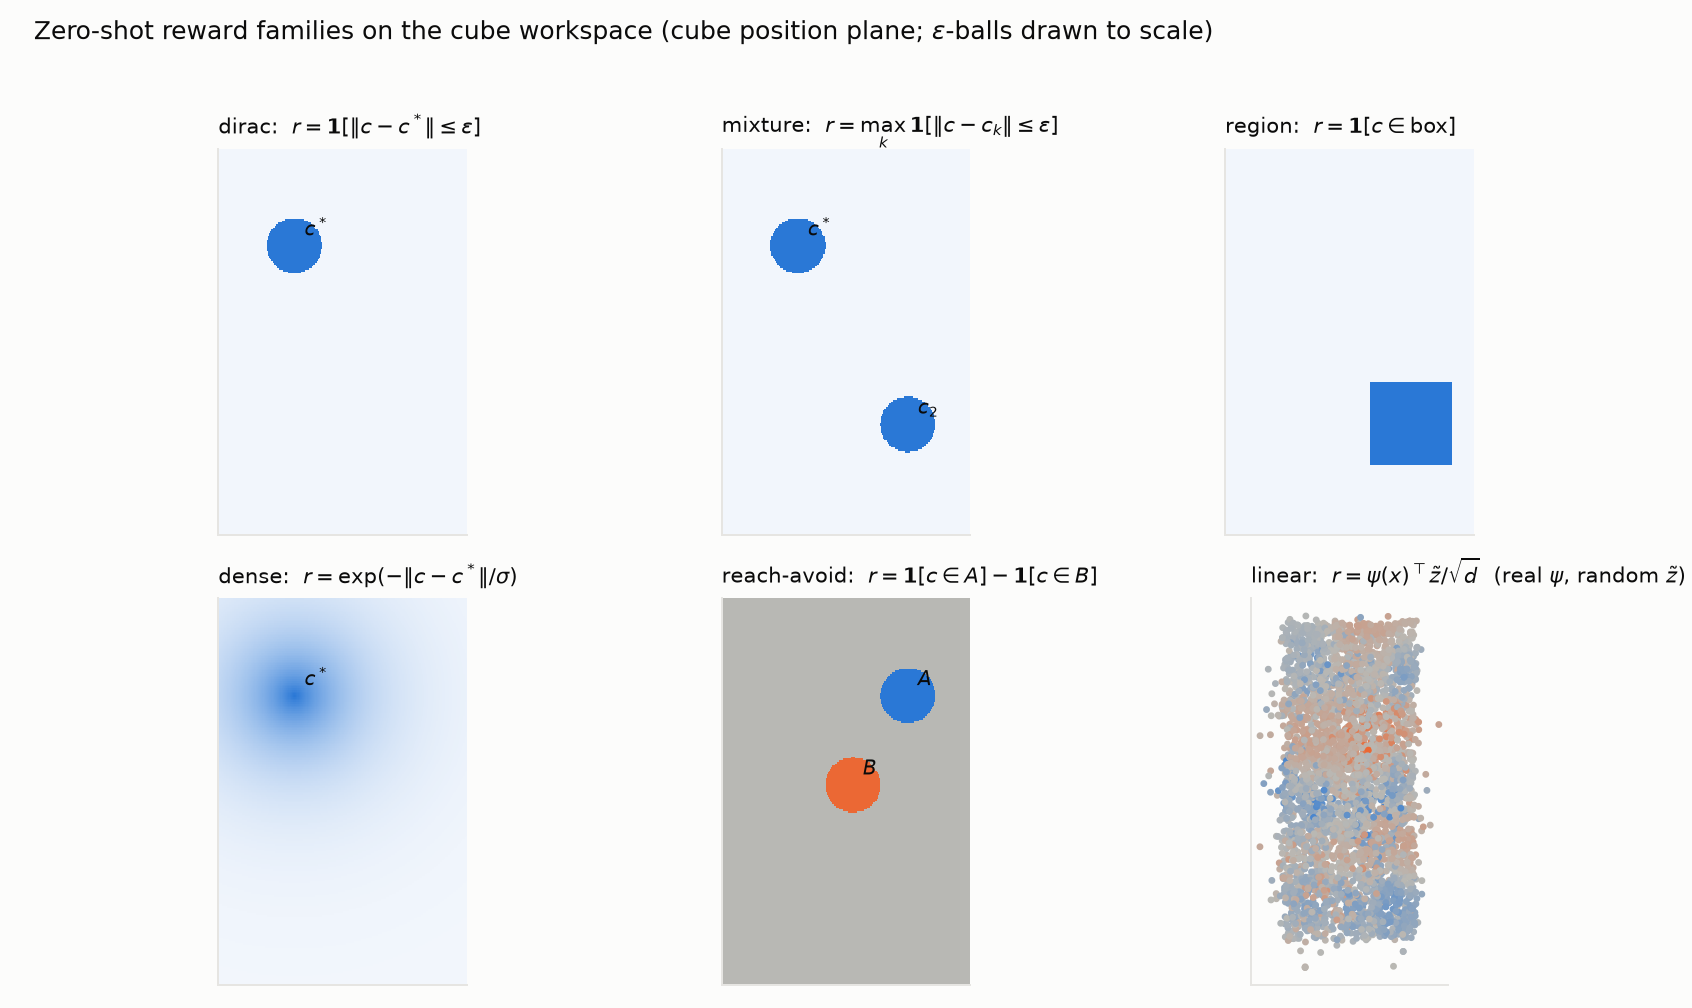
\includegraphics[width=0.95\textwidth]{figures/5_rewards.png}
\caption{The held-out reward families on the cube workspace (cube-position plane; $\epsilon$-balls to scale).
The first five panels are functions of cube position.
The \textsc{linear} panel colors dataset states by $\psi(x)^{\top}\tilde z$ for one random direction of the trained embedding: the field is spatially incoherent in cube space, which is the visual form of the coverage problem of \S\ref{sec:readout}.}
\label{fig:rewardfams}
\end{figure}

\label{app:rewards}

All transfer rewards are functions of the cube position $\cube(x)$, with centers drawn uniformly from dataset states; eight instances per family; all values in $[0,1]$.
\textsc{ball}~$\epsilon$ is
\begin{equation}
\ind{\|\cube(x)-c_0\|\le\epsilon}
\end{equation}
for
\begin{equation}
\epsilon\in\{0.4,0.8,1.6\}
\end{equation}
in observation units (the training kernel is $0.4$); \textsc{smooth}~$\sigma$ is
\begin{equation}
\exp(-\|\cube(x)-c_0\|^2/2\sigma^2)
\end{equation}
for
\begin{equation}
\sigma\in\{0.4,0.8\};
\end{equation}
\textsc{twozone} is
\begin{equation}
\max_k\ind{\|\cube(x)-c_k\|\le0.4}
\end{equation}
with
\begin{equation}
\|c_1-c_2\|>1.6.
\end{equation}
Inference uses $m=10{,}000$ relabeled rows.
Prediction is scored from $12$ teleported starts $\times$ $2$ rollouts; control over $10$ episodes per drive at horizon $200$, so returns lie in
\begin{equation}
[0,\sum_{t<200}\gamma^t]=[0,86.6].
\end{equation}
Table~\ref{tab:main}'s column groups average family means: concentrated $=$ \{\textsc{ball} $0.4$, \textsc{ball} $0.8$, \textsc{smooth} $0.4$\}, broad $=$ \{\textsc{ball} $1.6$, \textsc{smooth} $0.8$\}, compositional $=$ \textsc{twozone}.
Synthetic training rewards (\S\ref{sec:reward-transfer}) are drawn per batch: \textsc{kernel} mixes balls, Gaussians, and two-zone rewards with centers from the batch and log-uniform radii in $[0.2,2.0]$; \textsc{rff} draws
\begin{equation}
r=\mathrm{relu}(\cos(w^{\top}\cube+\varphi))
\end{equation}
with
\begin{equation}
w\sim\mathcal{N}(0,I)/b,
\end{equation}
\begin{equation}
\varphi\sim\mathrm{U}[0,2\pi).
\end{equation}
Both are normalized before reward inference.

\subsection{The two-stage procedure is not an exact factorization}
\label{app:twostage}

For a singleton goal, occupancy factors as first-arrival probability times a recurrence term.
For finite regions this identity fails: the region can be re-entered from many boundary states, so recurrence depends on where the region was entered and on the actions taken inside it.
Empirically, recurrence remains action-dependent on our data: across a grid of states, goals, and candidate actions, the intraclass correlation of recurrence across actions is $0.24$-$0.29$, far from the action-independence an exact factorization would need.
The two-stage procedure therefore uses phase 1 only to initialize phase 2, which optimizes occupancy directly with TD.

\subsection{Freezing one factor: relation to standard stabilization methods}
\label{app:freeze}

Holding part of a value function fixed while the rest trains appears in several standard forms.
Semi-gradient TD stops gradients through the bootstrap target \citep{sutton2018reinforcement}.
Deep value learning holds a target copy of the network fixed between synchronizations \citep{mnih2015human}, and DDPG trains its actor against a critic whose target copies move on a slower timescale \citep{lillicrap2016continuous}.
Two-timescale analyses of actor-critic make the requirement precise: convergence arguments hold when one component evolves slowly enough to appear stationary to the other \citep{borkar1997stochastic,konda2000actor}.
Successor-feature methods fix the feature map and train the other factor of a factored value function by TD \citep{barreto2017successor}.
Phase 2's freeze differs from all of these in one respect: the goal embedding is fixed for the entire phase rather than updated slowly, which is closest to the successor-feature setting.

\subsection{Derivations}
\label{app:derivations}

\paragraph{Proof of Proposition~\ref{prop:fixed-points}.}
\emph{No density:} a measure has a density with respect to $\rho$ only if it is absolutely continuous with respect to $\rho$.
The point mass
\begin{equation}
\delta_{f(s,a)}
\end{equation}
assigns mass $1$ to the set
\begin{equation}
\{f(s,a)\},
\end{equation}
which has $\rho$-measure zero when $\rho$ is non-atomic, so
\begin{equation}
\delta_{f(s,a)}\not\ll\rho
\end{equation}
and no Radon-Nikodym derivative exists.
\emph{Boundedness and contraction:} for measurable $G$ and deterministic dynamics,
\begin{equation}
P(G\mid s,a)=\ind{f(s,a)\in G}\in\{0,1\}.
\end{equation}
Both region operators act on bounded functions with the sup norm.
For the absorbing operator
\begin{equation}
(\mathcal{T}^{\Reach}Q)(s,a,g)=\E[h+\gamma(1-h)Q(s',a',g)]
\end{equation}
and any $Q_1,Q_2$,
\begin{equation*}
|\mathcal{T}^{\Reach}Q_1-\mathcal{T}^{\Reach}Q_2| \le\gamma\,\E[(1-h)\,|Q_1-Q_2|]\le\gamma\|Q_1-Q_2\|_\infty
\end{equation*}
since
\begin{equation}
0\le 1-h\le 1;
\end{equation}
the non-absorbing operator is a $\gamma$-contraction by the same bound without the
\begin{equation}
(1-h)
\end{equation}
factor.
Banach's fixed-point theorem gives a unique fixed point for each.
For the non-absorbing operator, unrolling the recursion and using the Markov property gives
\begin{equation*}
M(s,a,g)=\E[\sum_{t\ge0}\gamma^{t}h(s_{t+1},g)],
\end{equation*}
bounded by
\begin{equation}
1/(1-\gamma).
\end{equation}
For the absorbing operator, let
\begin{equation}
T_g=\min\{t\ge0:s_{t+1}\in B_\epsilon(g)\}
\end{equation}
and
\begin{equation}
Q^{*}=\E[\gamma^{T_g}\ind{T_g<\infty}].
\end{equation}
If
\begin{equation}
s_{1}\in B_\epsilon(g)
\end{equation}
then
\begin{equation}
T_g=0
\end{equation}
and the right side of the backup contributes
\begin{equation}
h=1=\gamma^{0};
\end{equation}
otherwise the backup contributes
\begin{equation}
\gamma\,\E[\gamma^{T_g'}\ind{T_g'<\infty}]
\end{equation}
with $T_g'$ the hitting time from $s_{1}$, and
\begin{equation}
T_g=T_g'+1
\end{equation}
on that event.
So $Q^{*}$ satisfies the fixed point equation, and by uniqueness it is the fixed point.
\hfill$\square$

\paragraph{The total-occupancy identity and its exactness conditions.}
For any start $(s,a)$, exchanging the expectation over goals with the sum over time,
\begin{equation*}
\E_{g\sim\rho}\!\left[\frac{M^{\pi}(s,a,B_\epsilon(g))}{N(g)}\right] =\E_{\pi}\Big[\sum_{t\ge0}\gamma^{t}\,w(s_{t+1})\Big], \qquad w(x):=\int_{B_\epsilon(x)}\frac{\rho(dg)}{N(g)},
\end{equation*}
using the symmetry
\begin{equation}
\ind{x\in B_\epsilon(g)}=\ind{g\in B_\epsilon(x)}.
\end{equation}
If goal regions partition the space (disjoint cells),
\begin{equation}
w\equiv1
\end{equation}
and the identity
\begin{equation}
\E_{g}[M/N]=1/(1-\gamma)
\end{equation}
is exact.
For overlapping balls,
\begin{equation}
w(x)=1
\end{equation}
whenever $N$ is constant on $B_\epsilon(x)$, so the identity holds to first order when $N$ varies slowly at scale $\epsilon$; and
\begin{equation}
\E_{x\sim\rho}[w(x)]=\int\rho(dg)\,N(g)/N(g)=1
\end{equation}
exactly by Fubini, so the identity is exact on average over states drawn from $\rho$.
The training penalty enforces the batch-mean form, which sits between these regimes.

\paragraph{The $1/N$ readout weight.}
Any reward's value is
\begin{equation}
Q_{r}(s,a)=\E_{x\sim\rho}[r(x)\,m(s,a,x)]
\end{equation}
with
\begin{equation}
m=dM/d\rho
\end{equation}
wherever the density exists.
The trained head outputs region mass,
\begin{equation*}
F^{\top}\psi(g)\approx M(s,a,B_\epsilon(g))=\int_{B_\epsilon(g)}m\,d\rho \approx m(s,a,g)\,N(g)
\end{equation*}
for $m$ approximately constant on the ball.
Hence
\begin{equation}
m(s,a,g)\approx F^{\top}\psi(g)/N(g)
\end{equation}
and
\begin{equation*}
Q_{r}(s,a)\approx\frac{1}{n}\sum_{j}r(g_{j})\,F^{\top}\psi(g_{j})/N(g_{j})
\end{equation*}
over goals $g_{j}\sim\rho$.
Omitting the
\begin{equation}
1/N(g_{j})
\end{equation}
factor multiplies the estimate by approximately
\begin{equation}
\bar N=\E[N]
\end{equation}
when $N$ is uncorrelated with $r\cdot m$ across goals, the
\begin{equation}
y=\bar N x
\end{equation}
line of Figure~\ref{fig:scale}.

\subsection{Monte-Carlo evaluation protocol}
\label{app:mc}

Teleport-style Monte-Carlo evaluation of the kind used in \S\ref{sec:set-calibration} must reset the environment before every rollout, not merely overwrite the simulator state: the episode step counter otherwise persists across rollouts and every rollout after the first truncates immediately, inflating model-to-Monte-Carlo ratios by one to two orders of magnitude.
A useful invariant when debugging such a harness: the implied total Monte-Carlo mass must approach
\begin{equation}
\sum_k\gamma^k,
\end{equation}
because the tracked object is always somewhere.

\end{document}